\section{Road Intersection Density}

As a novel approach for the distinction between formal and informal regions, we
propose the density of road intersections as a metric. This is based on the belief that areas can be characterized by the density of the road network. To illustrate, a dense road network would result in many intersections. The difference in density of intersections could indicate a different spatial organization between neighborhood. This could perhaps be used to detect the developing slums in our image data.

Road detection and extraction from satellite images is well established field of study with a large variety of developed methods \cite{mena2003state}.  The specific detection of road intersection is less studied although there are studies covering the subject \cite{hu2007road} \cite{koutaki2004automatic} as part of general road network extraction. 

\subsection{Convolutional Neural Network}

Since there is not a lot of research in the extraction of road network, we use the methods proposed in this field. After the roads are extracted from the image, we can use this road network to find the road intersections. A promising approach in road extraction is the use of Neural Networks \cite{mangala2011extraction} \cite{mokhtarzade2007road}. A study from 2017 was able to extract both the road network together with buildings with high accuracy using a Convolutional Neural Network \cite{alshehhi2017simultaneous}. We used the same approach a separate implementation of the convolutional neural network since the research paper did not include the software and data that was used in the study \cite{airs}. This implementation includes a open-source set of images, that was designed for the training and validation of the neural network \cite{MnihThesis}. After training on the provided images, the network was used to extract the roads from our own satellite images.  Unfortunately, the mask of the road network was erroneous as it did not represent the road network in the provided image. The suspected cause of this failure is the difference in the training data to our satellite imagery data. To illustrate, the trainingset contained satellite images obtained from mostly rural area's of the state of Massachusetts in the United States while the data used in our research is from Bangalore in India which is mostly urban. The geographical features and the road systems are quite different in the two areas. This is a probable cause for inability of the neural network to recognize the road network in the images from Bangalore. The difference in resolutions
of the two image sets could be another cause. The images of Massachusets were of quite a lower resolution than the images of Bangalore. This could have hindered correct classification as well, although this is ungrounded speculation.

\subsection{Hough Transform}
As an alternative to the neural network attempted to extract road networks using image processing methods. The image is subjected to a number of operations that extract the road network from the image. The first operation is the transformation of the RGB image to grayscale values. This is done in preparation for Otsu's method for threshold, which is able to separate buildings from roads \cite{otsu1979threshold}. The resulting image, displayed in Figure \ref{fig:roads_hough}, is a mask of the road network in the satellite image. From an aerial point of view, roads are straight lines of
constant width. The lines can be captured the using a Hough transform. The Hough transform is able to extract straight lines from images and create mathematical definition of the lines \cite{duda1972use}.  Once the roads are mathematically defined, determining the location of the intersection is straightforward.

\begin{figure}
\begin{tabular}{cc}
  \subfloat{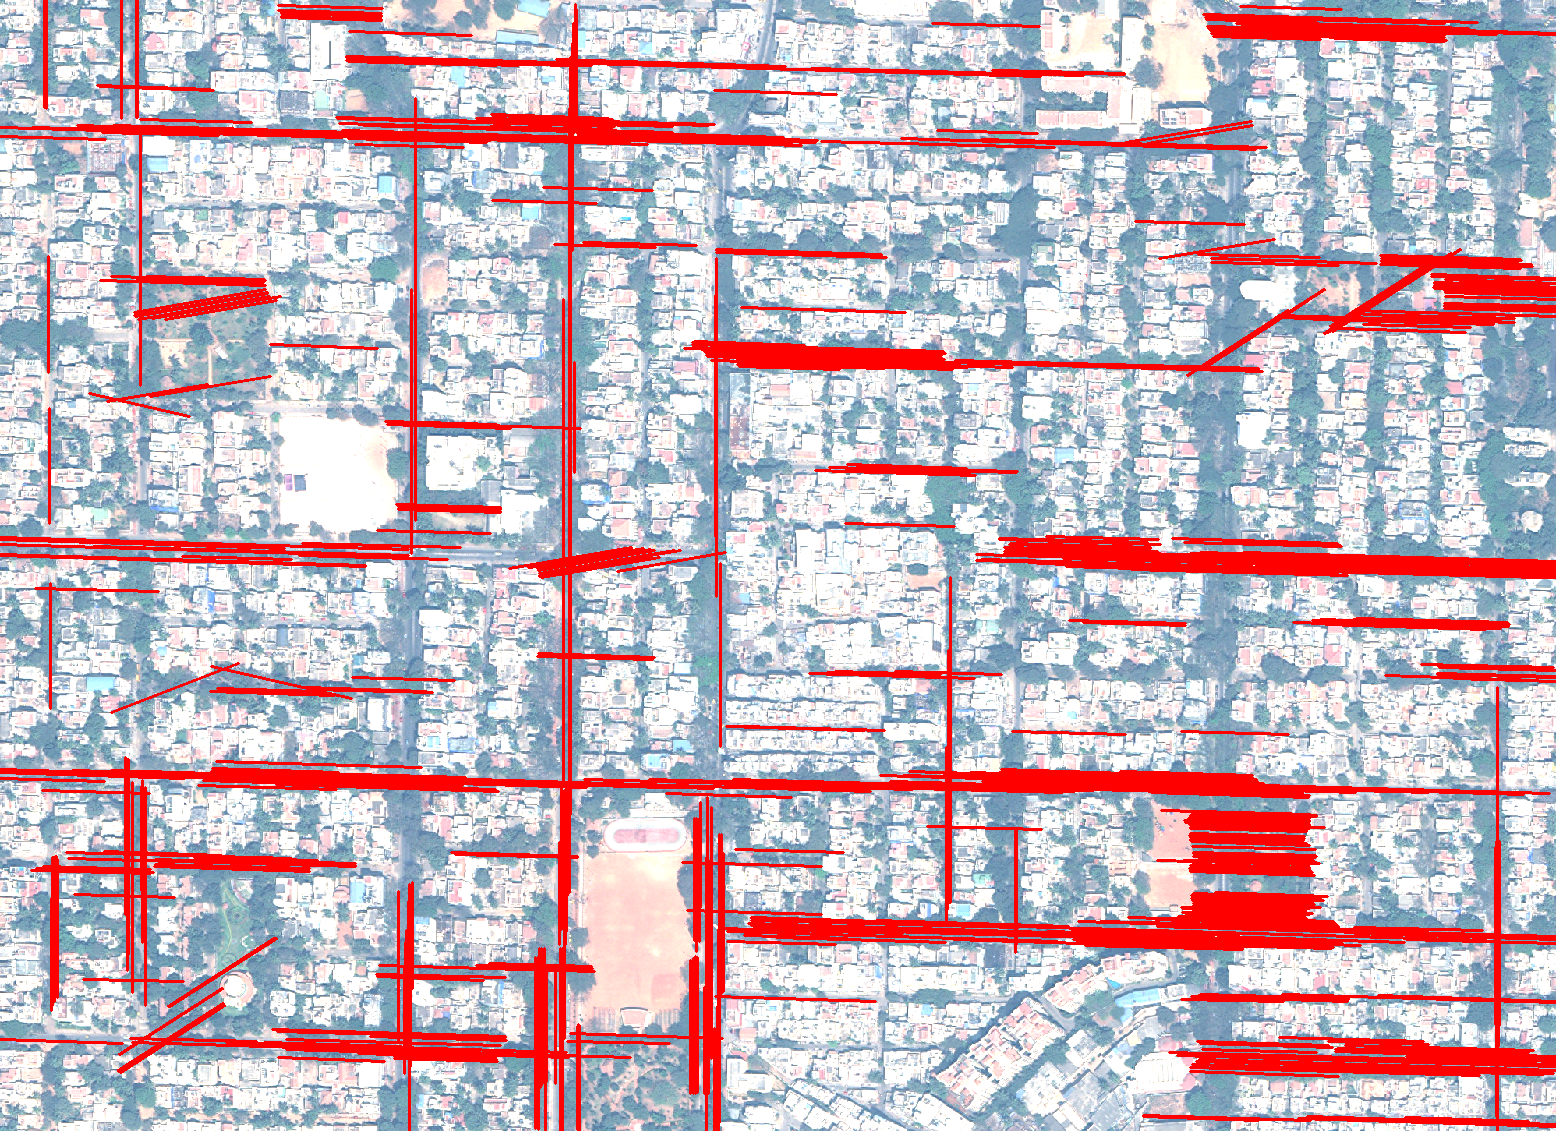
\includegraphics[width=7cm]{images/hough_road_section_8}}&
  \subfloat{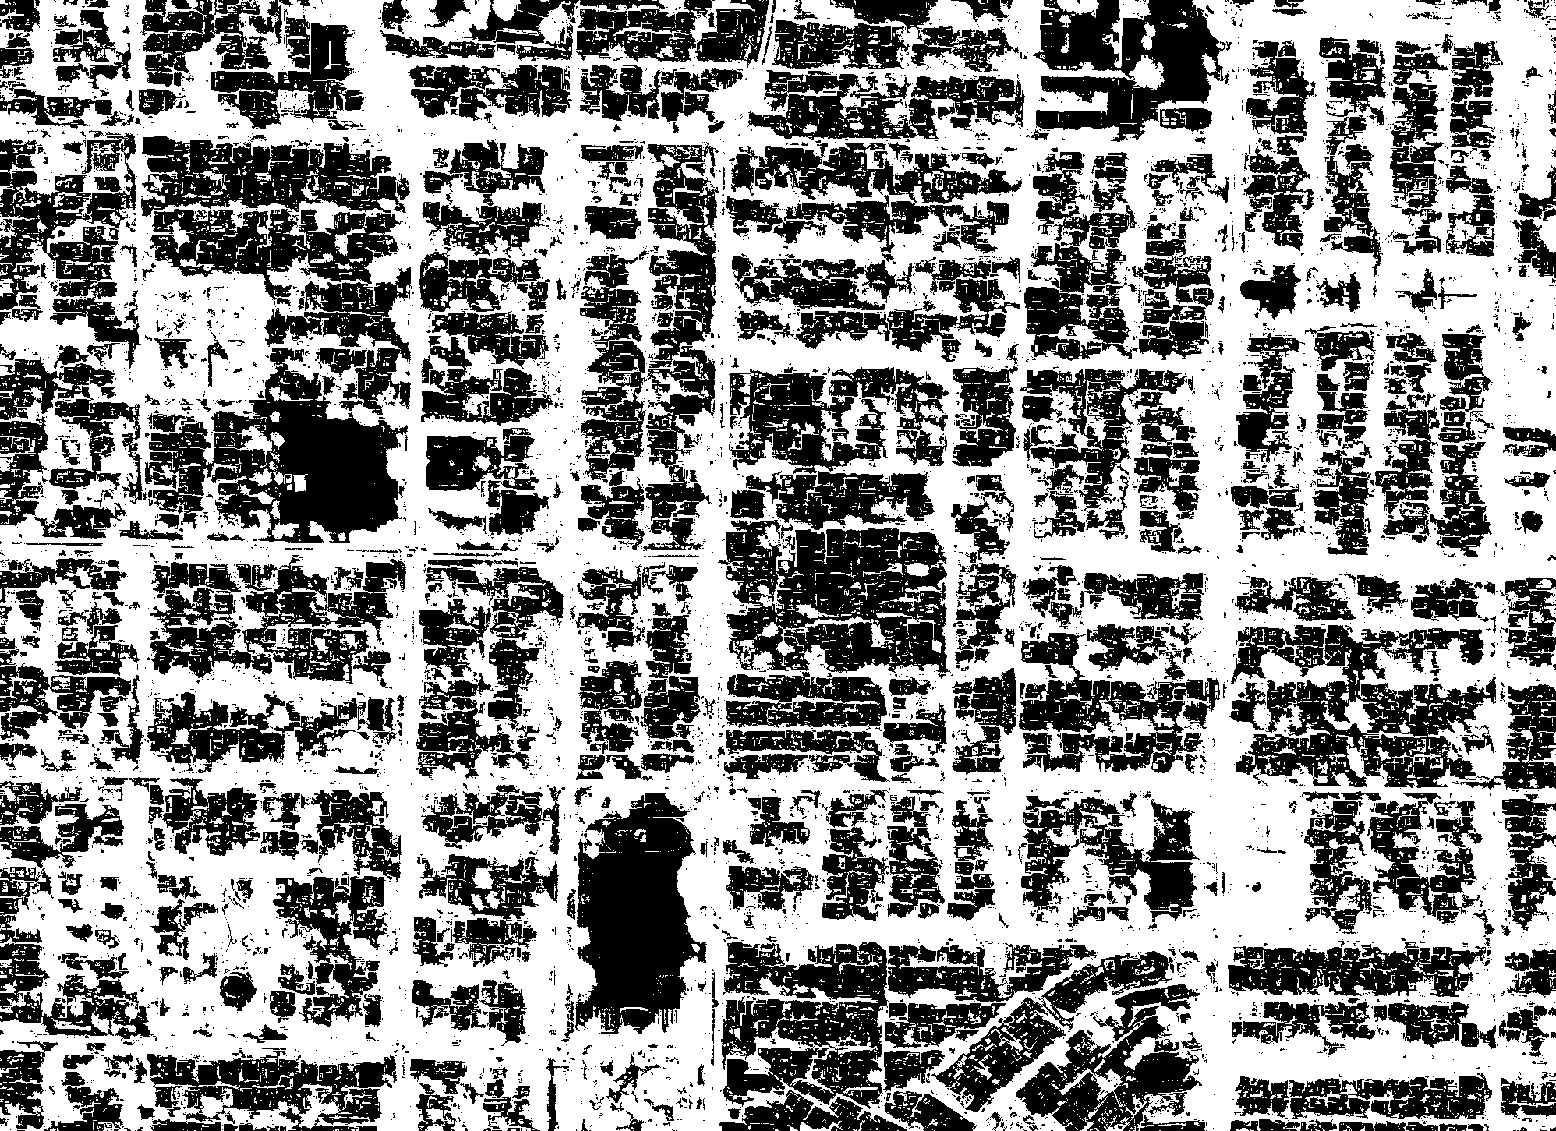
\includegraphics[width=7cm]{images/hough_road_section_8_mask}}
\end{tabular}
\caption{Detected roads using Otsu's thresholding method (left) combined with
Hough Transform (right)}
\label{fig:roads_hough}
\end{figure}

We implemented this approach in Python. The resulting mask and detected Hough lines are displayed in Figure \ref{fig:roads_hough}. This was the most balanced results we could get after changing the parameters for the creation of the mask and Hough lines. Different parameters would drastically increase recall and decrease accuracy beyond usefull application. In this case, the extracted mask  represents the road network quite accurately. The hough transform resulted in many correct lines, although there were a lot of duplicates and noise. Even though the noise and duplicates could be largely removed, we decided to pursuit a different method of intersection extraction. 

\subsection{Road Intersection Convolution}
We changed the approach of intersection detection to directly extract intersections from the satellite image. This is in contrast with the original approach, which first extracts the road network followed with the to detection of the intersections. In our new approach, we apply a convolution using a kernel in the shape of an cross directly on the satellite image. Because the kernel matches the shape of the intersection, the output of the convolution will have peaks in the output image on the positions of the intersections. The results from the proof of concept are displayed in Figure \ref{fig:roads_conv}. This approach is not entirely original, it has similarities to the use footprints to find the direction of intersections \cite{hu2007road}. That paper creates certain points, called seeds, in the image from which the road network expands using road segments. These roadsegments can be one of a few classes, for example, a straight road, T junction and cross intersection. The type depends on its surrounding pixels, which form a footprint that is classified as either one of the classes. Another study has a similar approach, which explicitly displays the different sizes of intersections \cite{koutaki2004automatic}. However, these two studies do not use convolution but different methods to match the footprints to the intersections in the image. The use of convolution is quite uncomplicated in comparison. For our purpose, the extraction of the orientation of an intersection is not important. We only require the location of intersections which is why a less complicated approach can be used.

\begin{figure}
	\begin{tabular}{cc}
		\subfloat{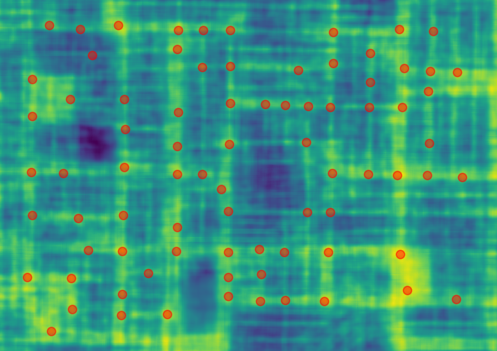
\includegraphics[width=7cm]{images/conv_road_section_8_1}}&
		\subfloat{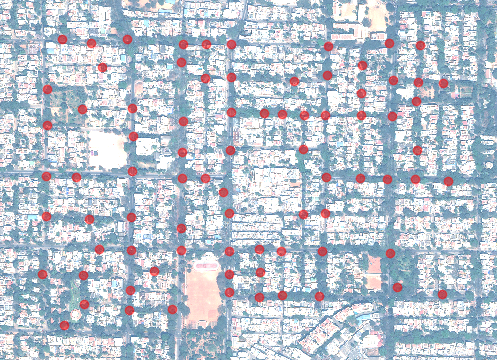
\includegraphics[width=7cm]{images/conv_road_section_8_2}}
	\end{tabular}
	\caption{Detection of intersections using convolution of a cross shaped kernel.
		Left: Heatmap of output of the convolution; Right: Located peaks overlayed on input image}
	\label{fig:roads_conv}
\end{figure}


Preceding the convolution, the satellite image is transformed to grayscale and subsequently inverted in color. In certain areas, the grayscale version of the image will already have a large contrast between roads and the surrounding buildings.  However, this in every image has this contrast. Therefore, we apply the Otsu's thresholding is after the transformation to grayscale. This creates a black and white version of the image with contrast between roads and buildings. 

The original kernel that was used as proof of concept is a n by n matrix, containing a cross of ones
with the remainder filled with zero's, as illustrated in Figure \ref{fig:conv_kernel} on the left. To clarify some terminology, the toe of an intersection is one of the roads leading to the
intersection. In the case of Figure \ref{fig:conv_kernel}, there are four toes
with a width and length two and three matrix cells, respectively. The width and length of a toe will also be referred to as the road width and length respectively. Theoretically, this kernel has the optimal activation when it is exactly located on the same shape of the kernel, thus cross intersections. It is therefore important to match the shape of the kernel to the shape of the intersections in the image. This means that the width of the toe in the kernel depends on the road width of the intersections in the image. Therefore, the dimension of the kernel depends on
the image used and the scale of the image. In practice, the values of the road width and length will be much higher than the values displayed in Figure \ref{fig:conv_kernel}. This is only a simple kernel for illustrative purposes. 

\begin{figure}%	
	\centering
	\begin{tabular}{cc}	
		{$\displaystyle
			\begin{pmatrix}
			0 & 0 & 0 & 1 & 1 & 0 & 0 & 0\\
			0 & 0 & 0 & 1 & 1 & 0 & 0 & 0\\
			0 & 0 & 0 & 1 & 1 & 0 & 0 & 0\\
			1 & 1 & 1 & 1 & 1 & 1 & 1 & 1\\
			1 & 1 & 1 & 1 & 1 & 1 & 1 & 1\\
			0 & 0 & 0 & 1 & 1 & 0 & 0 & 0\\
			0 & 0 & 0 & 1 & 1 & 0 & 0 & 0\\
			0 & 0 & 0 & 1 & 1 & 0 & 0 & 0
			\end{pmatrix}
			$} &
		$\vcenter{\hbox{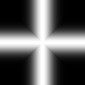
\includegraphics[width=4cm]{images/gauss_kernel}}}$
	\end{tabular}
	
	\caption{Left: Simple convolution kernel with a toe width and length of 2 and 3,
		respectively. Right: Gaussian convolution kernel}%
	\label{fig:conv_kernel}
\end{figure}

Figure \ref{fig:roads_conv} displays the results of the convolution
and the corresponding location of the detected peaks. The image used was a small section
of the image displayed in Figure \ref{fig:sections}d, not to be confused with the other three sections. It was chosen because of the width of the roads and the regularity of the road network with 90 degree angles between the toes of the intersection. Furthermore, the horizontal and vertical roads run parallel to the edges of the image. Moreover, the road network is quite distinct from
the background despite the vegetation covering a large part of the roads.

The peaks in the output of the convolution are located using local maxima detection from the Python scikit-image package \cite{scikit-image}. This function detects, as the name suggests, local maxima in an image. Local maxima are regions that stand out from surrounding area. The location of these maxima are the red dots displayed over the convolution and the corresponding input image in Figure \ref{fig:roads_conv}.

\subsubsection{Kernels}
In the development of this feature extraction method, we have designed multiple types of kernels to extract road intersections from images. In order create a increase accuracy of the intersections, we created a new type of kernel. This kernel is similar to the kernel in figure \ref{fig:conv_kernel}, but with the zero's replaced by negative numbers. The distance from the cross is proportional to the negative value of a cell in the kernel. This should only capture intersections, because when applied to areas which do not have the shape of a cross, the negative cells of the kernel should produce a large negative activation. However, applied in practice, this kernel also seems to be activated by intersection as well as straight sections of road. This unfortunately introduces many false positives.

To account for different widths of roads in an image, we created a kernel using Gaussian distributions, displayed in Figure \ref{fig:conv_kernel}. This kernel should smooth
the contrast between roads and roadside and might remove noise. As a result of
this kernel, the center of the road is the part that counts the most. The edges
of the road are less count for less, which should help make the kernel to a certain extend scalable
to multiple types and sizes of roads, such as alleys or main streets. We will therefore use this kernel by default.

\subsubsection{Intersection Detection Evaluation}

\begin{figure}
\begin{tabular}{cc}
  \subfloat{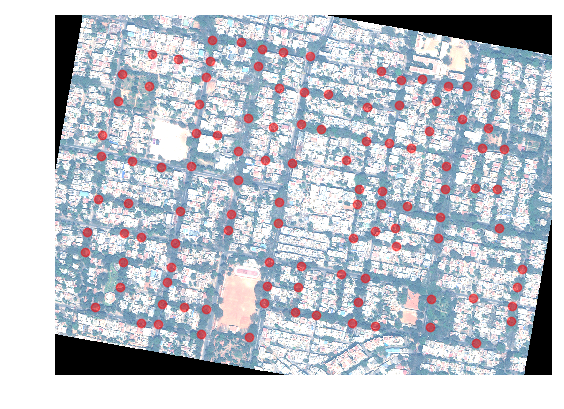
\includegraphics[width=7cm]{images/rot10}}&
  \subfloat{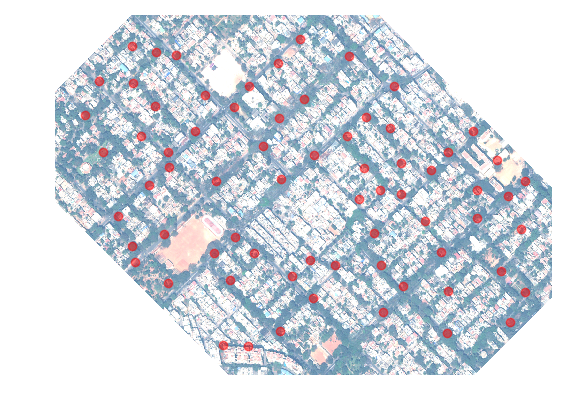
\includegraphics[width=7cm]{images/rot45}}
\end{tabular}
\caption{Performance of intersection detection in rotated intersections, from
  left to right with 10 and 45 degrees respectively}
\label{fig:roads_rot}
\end{figure}

A fundamental problem of this approach is the relation between the kernel and the resolution of the image. Increasing the scale or resolution of an image will
change the dimensions of the intersections. Because the content of the kernel
is required to match the intersections in the image in terms of pixels, the
dimensions of the kernel should change along with change in the image. Although
the usage of the Gaussian distribution creates a more versatile kernel, it is
still required to adjust parameters according to the resolution of the image.

Because of the fixed orientation of the cross in the kernel, this approach
should inherently be prone to differences in orientation. Therefore, in the
proof of concept, we used a road system with a constant orientation, as
displayed in Figure \ref{fig:roads_conv}. Because all intersections have the
same orientation, the kernel is able to detect a large number of intersections.
However, in many other areas, the road system is not nearly as consistent.
Intersections that are rotated relative to the orientation of the kernel should
therefore be more difficult to detect. To evaluate how well this approach performs with different orientations, we
applied a rotation of 10 degrees to the image displayed in Figure
\ref{fig:roads_conv}. In the resulting image, the fast majority of
intersections were still detected, as displayed in Figure \ref{fig:roads_rot}.
The increase of the rotation to the maximum of 45 degrees results in a loss of
detections, which is as expected. Surprisingly enough, there is almost no
increase in false positives. After analysis of the output of the convolution, we believe this seemingly
invariance to rotation is caused by the method of peaks detection.  When using
the rotated image, the resulting convoluted image is more smooth with less
peaks than the unrotated image. The local maxima detection is able to
correctly detect these faint peaks in the convoluted image. Although, this approach performs reasonably well under rotation, it should primarilty be used for images with minimal rotation.\newline

\noindent
As mentioned earlier, the road system displayed in figures \ref{fig:roads_conv} and \ref{fig:roads_rot} do not well represent the general road network encountered in the whole of the satellite image. This becomes apparent when observing the road system in the three section displayed in Figure \ref{fig:sections}. Although the majority of land area in these sections is formal, there is a clear contrast between these road systems and the road system used in the development of this feature. The road system in the three sections are much more narrow, shorter, and less regular than the road system in \ref{fig:roads_conv}. In these sections, on many occasions, even manual extraction of intersections is quite difficult. For instance, it is often not clear whether a part of the image between two buildings is an empty strip of land or actually a road. 

Due to the different nature of the road systems, parameters used to detect the intersections in Figure \ref{fig:roads_conv} and the sections in Figure \ref{fig:sections} are different. Because the streets in these three sections are generally more narrow and less long, both the road width and road length parameters are decreased relative to the parameters used in Figure \ref{fig:roads_conv}. Furthermore, the parameters for the local maxima detection are changed to only detect peaks that are really distinct from their surroundings. The motivation behind this is to reduce noise introduced by the irregularity and obscurity of the road network.

We could not perform a thorough objective evaluation of the intersection extraction due to the lack of a ground truth of the road intersections. Since we are not in the possession of a groundtruth, we cannot calculate objective measures for performance, such as accuracy, recall and the F1 score. Instead, the performance evaluation of the various methods and parameters used for the detection of intersection is based on subjective visual observation.

In conclusion, the use of a cross shaped kernel together with convolution seems to be able to extract the location of road intersections quite well. Although, for real world applications, such as road system mapping, this method for intersection detection might not be sophisticated enough. This method does not include the direction of the intersection. Furthermore, false positives and negatives are quite prevalent using this approach. This might meet not the performance achieved by different methods.

\subsection{Feature extraction}

\begin{figure}
	\begin{tabular}{cc}
		\subfloat{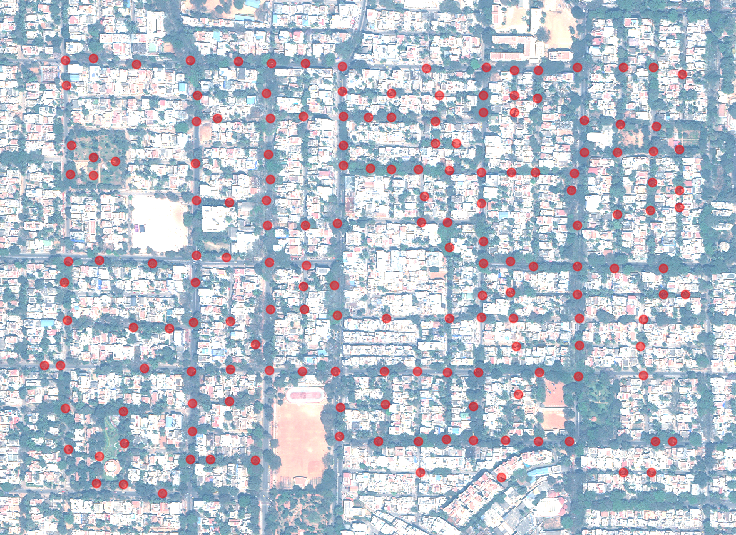
\includegraphics[width=7cm]{images/hotspotint}}&
		\subfloat{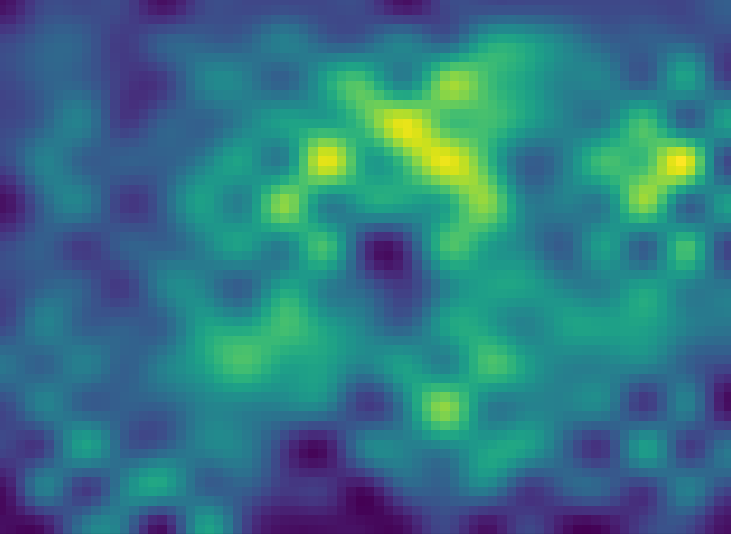
\includegraphics[width=7cm]{images/hotspot}}
	\end{tabular}
	\caption{Hotspots extracted from the detected intersections}
	\label{fig:roads_hotspot}
\end{figure}

The positions of the road intersections allow for the
feature extraction of the road density. Since the objective does not concern the
precise location the intersections of a region, misclassified or missed intersections are not of high concern, as long as the area is well represented by the correctly detected intersections. The density of road intersections in an area, is characterized by hotspot analysis using the Getis and Ord's local G function \cite{getis1992analysis}. The local G function is a meaure of spatial association between spatially distributed instance data. In our case, these instances are the locations of the intersections. The local G function is able to detect local hotspots and coldspots in instance data, effectively indicating the location of hotspots and coldspots of the density of intersections in the image of interest. This method for hotspot detection is implemented in the PySal python packackage \cite{rey2010pysal}. In order to create a feature from the local G function, the detected intersection need to be rasterized in the shape of the feature vector used in the other feature extraction methods. This rasterization allows for the feature to be easily combined with the features extracted from the satellite image using HoG and LSR. From this point on, we will refer to this feature extraction method as Road Intersection Density or RID.




